\documentclass[12pt,letterpaper,titlepage]{article}

\usepackage{fontspec}
\defaultfontfeatures{Mapping=tex-text}
\usepackage{xunicode}
\usepackage{xltxtra}
\usepackage{amsmath}
\usepackage{pdfpages}
\usepackage{amsfonts}
\usepackage{bbold}
\usepackage{amssymb}
\setcounter{secnumdepth}{0}
\usepackage{nameref}
\usepackage{enumitem}
\usepackage{environ}
\usepackage{pgfplots}
\usepackage{listings}

\showboxdepth=\maxdimen
\showboxbreadth=\maxdimen


\usepackage{paracol}
\usepackage{wrapfig}
\globalcounter{table}
\globalcounter{figure}
\usepackage{graphicx}
\usepackage[left=1in,right=1in,top=1in,bottom=1in]{geometry}
\graphicspath{{img/}}

\author{Jacob Abel}
\title{	Homework 4
	\\\large ECE2500 CRN:82943
}

\setlength{\parskip}{0.5em}

\begin{document}
\maketitle
\begin{raggedright}

\section{Single Cycle Data path}
\begin{center}
\includegraphics[width=\textwidth, height=\textheight, keepaspectratio=true]{single}

Implements \texttt{add, sub, beq, lw, sw, j} instructions
\end{center}

\clearpage

\paragraph{Problem 1: }
Consider the single-cycle data path given on the first page which implements the add, sub, \texttt{beq, lw, sw, j} instructions. Modify this data path to support the execution of a \texttt{bne} instruction, in addition to the other instructions already implemented. You are free to add/remove/modify multiplexers, ALU, adders, logic gates, shift units, and control signals. Your answer should consist of a concise description of the changes you will make to the data path as well as a figure that reflects the modified data path. You may draw only the part of the figure that is actually changed by your design.
\begin{center}
\includegraphics[width=0.75\textwidth, height=\textheight, keepaspectratio=true]{q1}

Modified Data Path

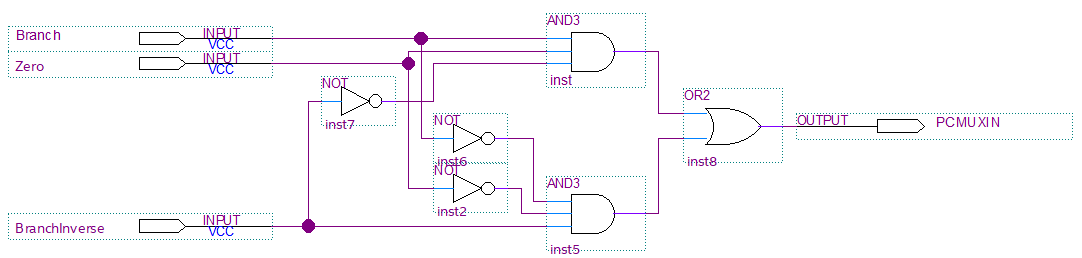
\includegraphics[width=0.75\textwidth, height=\textheight, keepaspectratio=true]{q1_0}

Added Component

\end{center}

The change is just replacing the and gate with a slightly more complex boolean logic circuit and adding a control out for when the branch comparison needs to be negated. The logic block guarantees that if there is a branch, the primary branch and inverse branch gates will never override each other.

\clearpage
\paragraph{Problem 2: }
Consider the execution of the following instructions in the modified
data path solved in Problem 1. For each instruction, write down the correct values for all the control signals \texttt{RegDst, Jump, Branch, MemRead, MemtoReg, ALUOp, MemWrite, ALUSrc, RegWrite}, and any control signal(s) added in Problem 1.

\begin{enumerate}
\item 
\begin{lstlisting}
sub $s0, $s1, $s2
\end{lstlisting}

\item 
\begin{lstlisting}
j 0xF43C
\end{lstlisting}

\item 
\begin{lstlisting}
lw $t0, 4($s1)
\end{lstlisting}

\item 
\begin{lstlisting}
bne $s0, $t0, LABEL
\end{lstlisting}
\end{enumerate}

All table entries in binary

\begin{tabular}{|l|c|c|c|c|c|}
  \hline Instruction      & \texttt{RegDst}   & \texttt{Jump}  & \texttt{Branch} 
       & \texttt{MemRead} & \texttt{MemtoReg}
\\\hline \texttt{sub \$s0, \$s1, \$s2}  & 1 & 0 & 0 & 0 & 0
\\\hline \texttt{j 0xF43C}              & X & 1 & X & 0 & X
\\\hline \texttt{lw \$t0, 4(\$s1)}      & X & 0 & 0 & 1 & 1
\\\hline \texttt{bne \$s0, \$t0, LABEL} & 0 & 0 & 1 & 0 & X
\\\hline
\end{tabular}

\begin{tabular}{|l|c|c|c|c|c|}
  \hline Instruction       & \texttt{ALUOp} & \texttt{MemWrite} & \texttt{ALUSrc}  
       & \texttt{RegWrite} & \texttt{BranchInverse}
\\\hline \texttt{sub \$s0, \$s1, \$s2}  & 10 & 0 & 0 & 1 & 0
\\\hline \texttt{j 0xF43C}              & XX & 0 & X & 0 & X
\\\hline \texttt{lw \$t0, 4(\$s1)}      & 00 & 0 & 1 & 1 & 0
\\\hline \texttt{bne \$s0, \$t0, LABEL} & 01 & 0 & 0 & 0 & 1
\\\hline
\end{tabular}
\clearpage

\paragraph{Problem 3: }
Imagine that you are a hardware designer who wants to add a new instruction to the MIPS ISA. Our new instruction has the following syntax: \texttt{lwr \$rd, \$rt(\$rs)}, the load word register instruction, which loads a word from memory into a destination register using a register as an offset (convenient!). Assume that we have found a way of encoding this instruction into 32-bit machine code using the R-type encoding format. We now want to modify the single-cycle data path in Figure 1 to support the execution of this instruction.

\begin{enumerate}
\item
Which new blocks (if any) do we need to add to support execution of this instruction? Please describe briefly and draw a figure to reflect the new design. Your goal must be to make minimum modifications to existing hardware.

A mux is added in between the mux and ALU input and a shift left 2 is added to this mux.

\begin{center}
\includegraphics[width=0.75\textwidth, height=\textheight, keepaspectratio=true]{q3a}

Modified Data Path
\end{center}


\pagebreak
\item
What new control signals (if any) do we need from the control unit to support this instruction?

RegIndr: Signifies a indirect + register offset

\item
Write the values for following control signals as well as any new control signals added: \texttt{RegDst, Jump, Branch, MemRead, MemtoReg, ALUOp, MemWrite, ALUSrc, RegWrite}.

All values listed in binary

\begin{description}
\item[RegDst] 1
\item[Jump] 0
\item[Branch] X
\item[MemRead] 1
\item[MemtoReg] 1
\item[ALUOp] 10 %Apply offset
\item[MemWrite] 0
\item[ALUSrc] 0
\item[RegWrite] 1
\item[RegIndr] 1
\end{description}

\end{enumerate}

\paragraph{Problem 4: }
Describe the advantages and disadvantages of single cycle versus pipelined data paths. Describe how changes (increases/decreases) in memory performance would affect each data path type.

Single cycle is much simpler and easy to design/debug. Additionally, as all instructions complete in one cycle, it is easy to program for as well. Unfortunately this also means that every instruction takes as long as the slowest instruction and you can't have multiple instructions computing at once (pipelining).

As memory is typically one of the slowest instructions, if you increase or decrease the memory speed, single cycle more or less directly increases/decreases in speed. In pipelined data paths, increasing/decreasing the memory speed will still increase/decrease the overall performance of the path but to a significantly smaller degree as in pipelined data paths, memory is not as much of a bottleneck.


\end{raggedright}
\end{document}